\documentclass[letter]{article}
\usepackage{tutorial}
\usepackage[OT1]{fontenc}

% ------------------------------------------------------------------------
\usepackage{graphicx}
\usepackage{subfigure}
\usepackage{epsfig}
\usepackage{psfrag}
% used to write c++ code/algorithms
\usepackage{listings}
\usepackage{fancyvrb}

%\psdraft

% hyperref stuff
\usepackage{hyperref}
\hypersetup{
  pdftitle={Getting started with CGAL Polyhedron},
  pdfauthor={INRIA Geometrica},
  pdfsubject={A tutorial for CGAL},
  pdfkeywords={},
  pdfpagemode=UseThumbs,
  baseurl={http://www.cgal.org},
  colorlinks=true,
  linkcolor=black,
  anchorcolor=black,
  citecolor=black,
  filecolor=black,
  menucolor=black,
  pagecolor=black,
  urlcolor=blue,
  bookmarksopen=false,}
% end hyperref stuff

\lstset{language=C++}

\graphicspath{{figs/}}
\def\figurename{Figure}
\def\tablename{Tableau}
\newcommand{\italic}[1]{\emph{#1}} 

% ------------------------------------------------------------------------
\newcommand\IL{{\itshape left}}
\newcommand\IR{{\itshape right}}
\newcommand\IM{{\itshape middle}}
\newcommand\IT{{\itshape top}}
\newcommand\IB{{\itshape bottom}}

% ------------------------------------------------------------------------
\def\kernel{\lstinline!Kernel!}

\def\cgalpoly{\lstinline!CGAL::Polyhedron_3!}
\def\poly{\lstinline!Polyhedron_3!}
\def\polytrait{\lstinline!PolyhedronTraits_3!}
\def\polyitem{\lstinline!PolyhedronItems_3!}
\def\polybuilder{\lstinline!Polyhedron_incremental_builder_3!}

\def\cgalhds{\lstinline!CGAL::HalfedgeDS!}
\def\hds{\lstinline!HalfedgeDS!}
\def\hdsitem{\lstinline!PolyhedronItems!}


\newcommand{\CodeFmt}[1]{{\small\texttt{#1}}}
\def\cgalpoly{\CodeFmt{Polyhedron\_3}}


% =========================================================================
\begin{document}

% TITLE
% ------------------------------------------------------------------------
\date{}
\title{{\LARGE {\sffamily\bfseries Getting started with CGAL Polyhedron}}}
% pierre: other suggestions for the title?
%  Mesh Processing with CGAL Polyhedron
%  Algorithms on Meshes with CGAL Polyhedron
%  Getting started with CGAL Polyhedron
% ?

\author{\small
\sffamily Le-Jeng Shiue\footnote{SurfLab, University of Florida}
\and \small
\sffamily Pierre Alliez\footnote{GEOMETRICA, INRIA Sophia-Antipolis}
\and \small
\sffamily Radu Ursu\footnote{GEOMETRICA, INRIA Sophia-Antipolis}
\and \small
\sffamily Lutz Kettner\footnote{MPII, Saarbr\"ucken}}
\maketitle

\thispagestyle{empty}

% ABSTRACT
% ------------------------------------------------------------------------
\abstract{
This document is a tutorial on how to get
started with the polyhedron data structure
provided by the Computational Geometry 
Algorithm Library (CGAL). Assuming the reader to be
familiar with the C++ template mechanisms and the 
key concepts of the generic programming, the tutorial is 
organized as the development process of a meshing application. 
The tutorial starts with a mesh viewer which holds a 
default polyhedron then a customized polyhedron.
The customized polyhedron contains the algorithmic flags
of the vertices, halfedges and facets. The mesh viewer 
demonstrates some basic manipulations of the polyhedron.
Subdivisions are the meshing algorithms in our meshing
application. The tutorial demonstrates how to implement 
subdivisions. Three different approaches are proposed with 
increasing level of sophistication and abstraction of implementing
subdivisions. The simplest approach uses the operators 
of the combinatorial modifications to implement 
the $\sqrt{3}$ subdivision scheme. 
A second approach overloads the modifier, with the help 
of the incremental builder, to implement 
the quad-triangle subdivision. The third approach abstracts 
the geometry operations from the refinements.
This approach offers a convenient way to specialize a subdivision with
the template geometry rules. Catmull-Clark, Loop and Doo-Sabin
subdivisions are illustrated using the latter approach. 
}
%%\vskip 3mm

%% \noindent {\bf Keywords:}
%%                  CGAL library,
%%                  tutorial,
%%                  halfedge data structure, 
%%                  polygon surface mesh,
%%                  subdivision surfaces,
%%                  quad-triangle,
%%                  $\sqrt{3}$,
%%                  Loop,
%%                  Doo-Sabin,
%%                  Catmull-Clark,
%%                  OpenGL.

\begin{center} 
  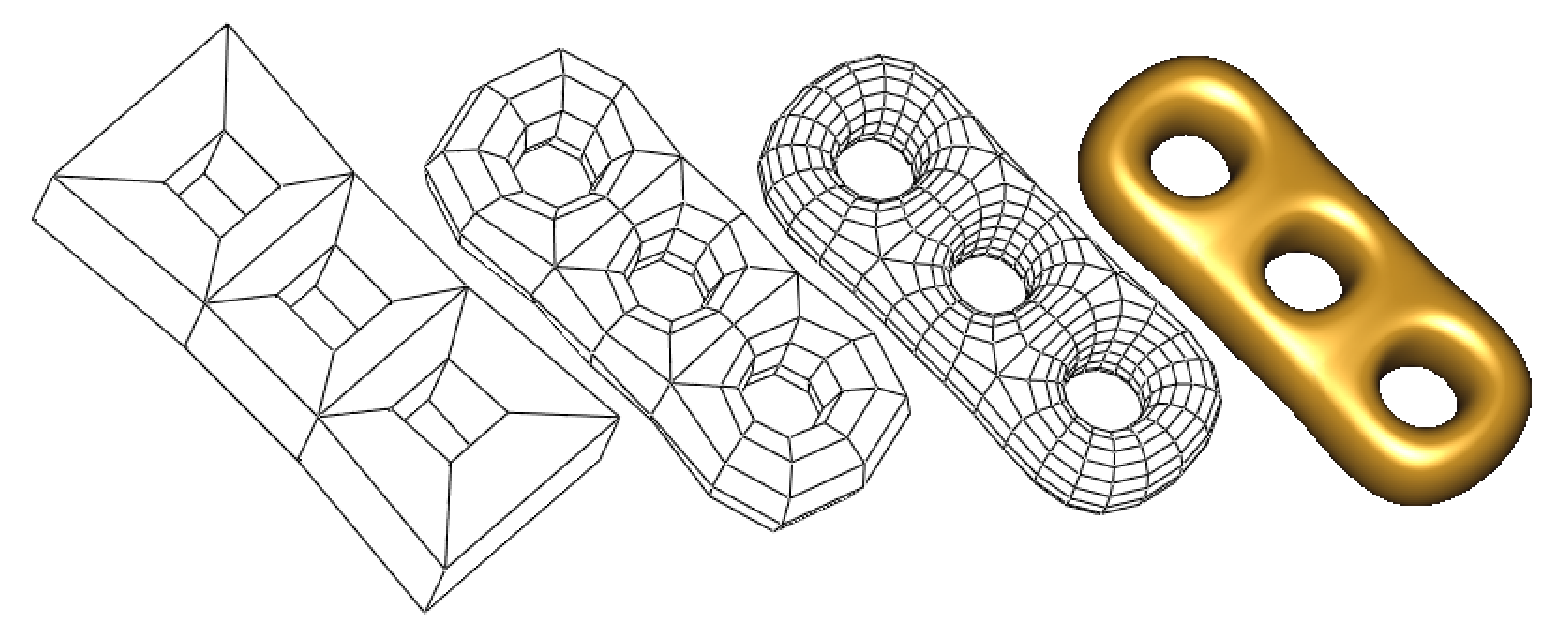
\includegraphics[width=12.0cm]{figs/teaser}\\
{\scriptsize Demo application running on Windows. A polygon mesh is 
   subdivided using the quad-triangle subdivision scheme.}

\end{center}

Polyhedron data structures based on the concept of
\emph{halfedges} have been very successful for the design
of general algorithms on meshes. 
Although making a preliminary version of a halfedge-based mesh data
structure is as a fairly simple task and is often proposed as a
programming exercise, the time has come where we should not write our
own mesh data structure from scratch anymore. With the emerging of
the generic programming in C++, a set of reusable library
components for graphics modeling and geometry processing are demanded
by researchers and developers. \emph{Extensible algorithm} models based on
a \emph{robust, efficient and customizable polyhedron 
data structure} will certainly speed up
the research as well as the development cycle, and benefit the 
community of the graphics modeling and geometry processing.  

Most of mesh algorithms employ a customized 
halfedge data structures and most of the customizations 
are specialized by customizing the primitive data, 
which are the vertex positions, the facet normals or other 
algorithmic flags. \cgalpoly\ encapsulates a generic
design of the halfedge data structure allowing users
customize the \poly\ with the template parameters of
the geometry primitives. There are several advantages
that employing the \poly\ as the core data structure
of a meshing application: \\
\indent $\bullet$ The \poly\ is a generic data structure which 
is customizable.
\indent $\bullet$ The \poly\ is a \emph{robust} and \emph{optimized} 
data structure.\\
\indent $\bullet$ A complete set of the geometry entities and predications 
is provided within CGAL.\\
\indent $\bullet$ CGAL is standardized following the C++ STL.\\

We have designed and implemented a meshing application
based on the \cgalpoly . This program provides a
mesh viewer supporting file I/O, mesh rendering 
and trackball manipulation and is accompanied with a set of 
subdivision algorithms. This tutorial instructs
the readers through the design and the implementation of the 
program. The first part of the 
tutorial highlights the design and implementation issues 
related to the \poly\ of the viewer. The second part
of the tutorial explains how to implement 
the connectivity and geometry operations of the 
subdivision algorithms. The source codes are 
published with the tutorial and can be accessed at ??.

The tutorial starts with demonstrating
how to implement a simple viewer based on the default
configuration of the \cgalpoly . This simple viewer 
demonstrates some basic functionalities of the \cgalpoly\ such as
\emph{modifier} and \emph{incremental builder} for initialization and 
the mesh traversal, i.e. the \emph{iterators} and the \emph{circulators},
for rendering or mesh exporting. Based on this simple
viewer, this tutorial then demonstrates
the \emph{customization of the \poly}. With primitives 
specialized with the algorithmic flags, an enriched polyhedron
is proposed and used as the core data structure of 
the meshing application. The tutorial then show how
to interact a customized \poly . The extended primitives
flags are employed to support the superimposition of the 
input mesh on the subdivided surfaces. A trackball function
of the enriched polyhedron is also dmonstrated in the tutorial.

The second part of the tutorial focuses on the design and 
the implementation of the subdivision algorithms.
In addition to the importance in surface modeling,
we choose subdivision algorithms to demonstrate
both the \emph{topology operation} (refinement) and the 
\emph{geometry operations} (smoothing). The topology and the geometry
operations are the two basic operations required by
most geometry algorithms. Our implementations of the subdivisions 
are designed to be a separated library that accept 
any generic \poly\ as the input polyhedron (not just the enriched polyhedron
we used in the mesh viewer). The key to implement
a subdivision scheme is to support the refinement, 
i.e.\ the connectivity modifications.
Two approaches are first introduced to support the refinement:
the \emph{atomic operators of the combinatorial modifications}
(operator scheme) and the \emph{modifier mechanism} (modifier scheme).
The operator scheme reconfigures
the connectivity with a combination of several combinatorial 
operators. The $\sqrt{3}$ subdivision is used to demonstrate this scheme.
Though simple and efficient in some refinements, e.g.\ $\sqrt{3}$ 
subdivision, the correct combination of the operators is 
hard to find for some refinements, 
e.g.\ Doo-Sabin subdivision. The modifier scheme
solves the problem by letting the programmers 
create their own combinatorial operators
using the polyhedron incremental builder.
The Quad-Triangle subdivision is used to demonstrate this scheme.

Subdivisions can be represented
as a combination of a refinement and a set of smoothing
rules. Based on this observation, our third approach 
generalizes the subdivision by abstracting the smoothing rules
from the refinement. The refinement is designed as a \emph{host 
function} that accepts a \emph{policy class} supporting the 
smoothing rules. A subdivision function is then a 
legal combination of the refinement and the smoothing rules.
This approach offers a convenient way to specialize a subdivision 
with the \emph{template smoothing rules}.
Catmull-Clark, Loop and Doo-Sabin
subdivisions are illustrated using the latter approach. 

The intended audience of this tutorial are researchers, 
developers or students in the graphics community developing 
algorithms around meshes. Experiences on the advance C++
design (i.e.\ generic programming using templates) and
knowledge of the halfedge data structure and 
subdivisions are prerequisites. 

\end{document}
